%!TEX root = main.tex
\section{Final Evaluation Study: Methodology and Results} \label{evaluation}
\par Our final evaluation study addresses RQ3 and RQ4---whether our new and improved VQS helps accelerate insight, and how it could fit into real analysis workflows. Participants for the evaluation study were recruited from each of the three aforementioned research groups, as well as domain-specific mailing lists. Prior to the study, we asked the potential participants to fill out a pre-study survey to determine their eligibility. Eligibility criteria included: being an active researcher in the subject area with more than one year of research experience, and having worked on a research project involving data of the same nature as that used in the participatory design. Four of the user studies were conducted remotely.  
\par Participants had the option of exploring their own dataset or an existing dataset that they provided to us during the participatory design process. All three blank-slate participants opted to explore their own datasets. After loading their dataset, we emailed them a screenshot of a visualization from our tool to verify that we configured the system to meet their needs. 
\par At the start, participants were provided with an interactive walk-through explaining the details of the features offered in our VQS. The participants were then given approximately ten minutes to experience a guided exploration of our VQS with a preloaded real-estate example dataset from Zillow \cite{zillow}.\notvcgTR{This dataset contained housing data for various cities, metropolitan areas, and states in the U.S. from 2004-15.} After familiarizing themselves with the tool, we loaded the participant's dataset and suggested an appropriate choice of axis to begin the exploration. Participants were encouraged to talk-aloud during the data exploration phase.
\par During the exploration phase, participants were informed that they could use other tools as needed. If the participant was out of ideas\ccut{ for three minutes}, we suggested one of the ten main functionalities in \zv \notvcgTR{\footnote{query by sketching, drag-and-drop, pattern loading, input equations, representative and outliers, narrow/ignore x-range options, filtering, data smoothing, creating dynamic classes,  data export}}that they had not yet covered. If any of these operations were not applicable to their specific dataset, they were allowed to skip the operation after having considered how it may or may not be applicable to their workflow. The user study ended after they covered all ten main functionalities. On average, the main exploration phase lasted for 63 minutes. After the study, we asked them open-ended questions about their experience. 
%%%%%%%%%%%%%%%%%%%%%%%%%%%%%%%
\subsection{Data Collection \& Analysis}
We recorded audio, video screen captures, and click-stream logs of the participant's actions during the evaluation study. We analyzed the transcriptions of these recordings \tvcg{through open-coding and
categorized every event in the user study using the coding labels:} 
\begin{denselist}
    \item Insight (Science) \textbf{[IS]}: Insight that connected back to the science (e.g. ``This cluster resembles a repressed gene.'')
    \item Insight (Data) \textbf{[ID]}: Data-related insights (e.g. ``A bug in my data cleaning code generated this peak artifact.'')
    \item Provoke (Science) \textbf{[PS]}: Interactions or observations made while using the VQS that provoked a scientific hypothesis to be generated.
    \item Provoke (Data) \textbf{[PD]}: Interactions or observations made while using the VQS that provoked further data actions to continue the investigation.
    \item Confusion \textbf{[C]}: Participants were confused during this part of the analysis.
    \item Want \textbf{[W]}: Additional features that participant wants, which is not currently available on the system.
    \item External Tools \textbf{[E]}: The use of external tools outside of \zv to complement the analysis process.
\end{denselist}
\npar In addition, \tvcg{based on the usage of each feature during the user study, we categorized the features into one of the three usage types:} 
\begin{denselist}
    \item Practical usage \textbf{[P]}: Features used in a sensible and meaningful way.
    \item Envisioned usage \textbf{[E]}: Features which could be used practically if the envisioned data was available or if they conducted downstream analysis, but was not performed due to the limited time during the user study. 
    \item \tvcg{Not useful \textbf{[N]}: Features that are not useful or do not make sense for the participant's research question and dataset.}
\end{denselist}
\tvcg{We chose to derive these labels from the user study transcription rather than through self-reporting to circumvent the bias that users may have when self-reporting, which can often artificially inflate the usefulness of the feature or tool under examination.} %\dor{Added based on Hidy's feedback.}}

\begin{figure}[ht!]
    \centering
    \vspace{-10pt}
    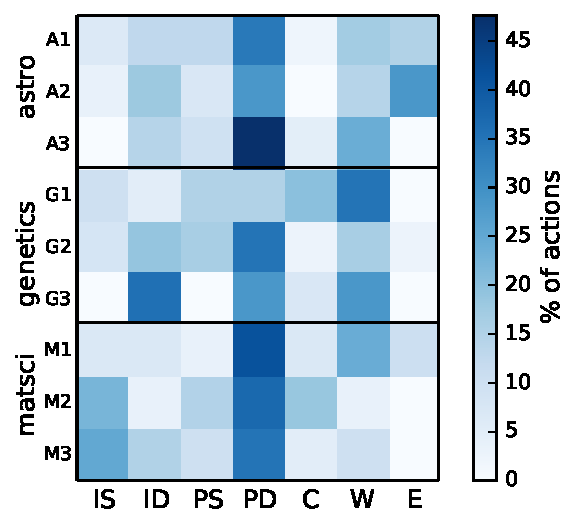
\includegraphics[width=0.7\columnwidth]{figures/result1.pdf}
    \vspace{-6pt}\caption{Heatmap \tvcg{showing percentage of participants' actions on \zv falling under each thematic encoding category.} \zv provokes participants to perform many data actions \textbf{[PD]} and generate scientific hypothesis \textbf{[PS]}. Occasionally, the series of data operations and hypothesis can lead to an scientific \textbf{[IS]} or data-related insight \textbf{[ID]}.}
    \vspace{-10pt}
    \label{action_heatmap}
\end{figure} 

\begin{figure}[ht!]
    \centering
    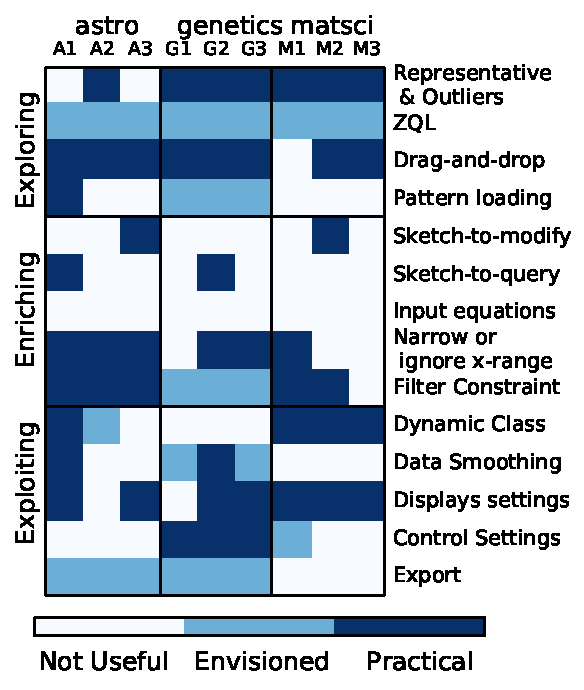
\includegraphics[width=0.7\columnwidth]{figures/result2.pdf}
    \vspace{-6pt}\caption{Heatmap of features categorized as practical usage (P), envisioned usage (E), and not useful (N). We find that participants preferred to query using bottom-up methods such as drag-and-drop over top-down approaches such as sketching or input equations. Participants found that data faceting via filter constraints and dynamic class creation were powerful ways to compare between subgroups or filtered subsets. The columns are arranged in the order of subject areas and the features are arranged in the order of the three foraging acts.}
    \label{feature_heatmap}
    \vspace{-5pt}
\end{figure}

\par The audio recordings and transcriptions of pre- and post-study interview questions are thematically encoded and summarized in Figure \ref{action_heatmap} and \ref{feature_heatmap}. Our study results fall into two main themes, which will be discussed in subsequent sections. First, we discuss how VQS features were used in practice to achieve scientific insights (RQ3). We find that VQSs can enable rapid, fluid iteration, catalyzing new questions or insights; that different querying modalities in VQSs support different forms of exploration; and that expressive querying allowed participants to compose novel analysis patterns. Second, we determine where VQSs fit into real data analysis workflows (RQ4). We find that VQSs can be used for a range of tasks that go beyond just exploration; that participants used the outputs from VQSs in various ways; and that VQSs are most appropriate for certain types of datasets.
